\section{Chia sẻ dữ liệu giữa các ứng dụng}

  Trong hệ điều hành Android, mỗi ứng dụng khi được cài đặt sẽ hoạt động như một thực thể độc lập, được bảo vệ bằng cơ chế sandbox. Cơ chế này ngăn cản ứng dụng truy cập trực tiếp vào dữ liệu của ứng dụng khác, giúp nâng cao tính bảo mật và quyền riêng tư cho người dùng. Tuy nhiên, trong một số tình huống thực tế, các ứng dụng vẫn cần khả năng chia sẻ dữ liệu cho nhau. Ví dụ, một ứng dụng chỉnh sửa ảnh có thể cần truy cập đến bộ sưu tập ảnh, hoặc một ứng dụng mạng xã hội cần truy cập danh bạ để đề xuất kết bạn. Để hỗ trợ nhu cầu này mà vẫn đảm bảo an toàn, Android cung cấp một số cơ chế chuẩn để chia sẻ dữ liệu giữa các ứng dụng một cách kiểm soát và có chọn lọc.

% 3.1
\subsection{Cơ chế dùng chung User-id}
\renewcommand{\labelitemi}{--}    
        Đây là một điểm trong bảo mật và cấp quyền của Android Các ứng dụng Android có thể dùng chung user-id nếu có cùng chứng chỉ số(digital certificate):
        \setlength{\leftmargini}{1.5cm}
        \begin{itemize}
            \item Mặc định khi một ứng dụng được cài đặt, hệ điều hành Android sẽ tạo một UID (User ID) riêng biệt cho nó, mỗi app chỉ có thể truy cập tài nguyên của chính nó (sandbox).
            \item Hai hoặc nhiều ứng dụng có thể dùng chung UID nếu chúng được ký bằng cùng một khóa chứng thực số (digital certificate) và chúng khai báo "android:shared UID" giống nhau trong AndroidManifest.xml.
            \item Yêu cầu bắt buộc là chứng chỉ số giống nhau, Android dùng digital signature để đảm bảo chỉ các app thuộc cùng một nhà phát triển mới có thể chia sẻ UID. Điều này ngăn chặn app lạ cố tình khai báo sharedUserId để xâm nhập dữ liệu của app khác.
            Ví dụ nếu app A và app B có sharedUserId giống nhau nhưng ký bằng chứng chỉ khác nhau do đó hệ thống từ chối cài đặt!
            \item Lợi ích là các app có thể truy cập dữ liệu và file của nhau, có thể dùng chung database, file cấu hình…, có thể chia sẻ quyền như đọc SMS, camera… nếu quyền được cấp.
        \end{itemize}
% 3.2
\subsection{ContentProvider và Intent}    
        Một trong những cơ chế chia sẻ dữ liệu quan trọng nhất trong Android là ContentProvider \cite{Content-Providers}. Đây là một lớp trung gian cho phép một ứng dụng cung cấp quyền truy cập có kiểm soát đến dữ liệu của mình cho các ứng dụng khác. ContentProvider hoạt động giống như một cơ sở dữ liệu với API chuẩn, cho phép các ứng dụng khác thực hiện thao tác như đọc, ghi, sửa hoặc xóa thông tin, nhưng chỉ trong phạm vi mà nhà phát triển cho phép. Ví dụ điển hình là ứng dụng Danh bạ của Android – nó triển khai một ContentProvider cho phép các ứng dụng khác như Zalo, Facebook hay Viber truy xuất thông tin liên lạc, nhưng chỉ sau khi người dùng đồng ý cấp quyền.

        \vspace{0.5em}

        Ngoài ContentProvider, Android còn hỗ trợ chia sẻ dữ liệu thông qua các Intent. Intent là một cơ chế giao tiếp giữa các thành phần trong Android, có thể được sử dụng để truyền dữ liệu giữa các Activity, Service, hoặc giữa các ứng dụng khác nhau. Khi một ứng dụng muốn gửi một tập tin, một đoạn văn bản, hình ảnh hoặc bất kỳ dữ liệu nào sang ứng dụng khác (ví dụ như chia sẻ ảnh lên mạng xã hội), nó có thể tạo một Intent có chứa dữ liệu và gọi startActivity hoặc startActivityForResult. Ứng dụng nhận dữ liệu sẽ phải khai báo rõ ràng trong AndroidManifest.xml các intent filter phù hợp để có thể tiếp nhận loại dữ liệu đó. Cơ chế này đơn giản, phổ biến, và rất hiệu quả cho các thao tác chia sẻ ngắn hạn, không yêu cầu truy cập thường xuyên.

        \vspace{0.5em}

        Một phương pháp khác nữa là sử dụng bộ nhớ ngoài (external storage), tức là các file được lưu trên thẻ nhớ hoặc phân vùng có thể truy cập công khai. Trước đây, bất kỳ ứng dụng nào có quyền đọc/ghi vào bộ nhớ ngoài đều có thể truy cập dữ liệu của ứng dụng khác lưu ở đó. Tuy nhiên, kể từ Android 10 (API 29), Google đã giới thiệu cơ chế Scoped Storage để hạn chế quyền truy cập tự do này. Scoped Storage yêu cầu ứng dụng chỉ có thể truy cập vào thư mục riêng của mình trên bộ nhớ ngoài hoặc các file cụ thể được chia sẻ thông qua MediaStore hoặc Storage Access Framework.

% 3.3
\subsection{FileProvider}
\renewcommand{\labelitemi}{--}   

      Một cách hiện đại và an toàn để chia sẻ dữ liệu giữa ứng dụng là sử dụng các API do hệ thống quản lý như FileProvider. Đây là một lớp đặc biệt giúp ứng dụng có thể chia sẻ tệp tin thông qua URI mà không cần cấp quyền truy cập bộ nhớ ngoài toàn cục. FileProvider chỉ cấp quyền truy cập tạm thời, đúng với tệp mà ứng dụng chia sẻ, và chỉ dành cho ứng dụng nhận cụ thể trong một khoảng thời gian nhất định. Điều này giúp tránh được việc ứng dụng khác có thể lén đọc toàn bộ dữ liệu người dùng mà không được cho phép \cite{FileProvider}.

      \vspace{0.5em}

      Tóm lại, Android cung cấp nhiều phương thức để chia sẻ dữ liệu giữa các ứng dụng, mỗi phương thức phù hợp với từng nhu cầu khác nhau. Tuy nhiên, tất cả các cơ chế này đều được thiết kế với tiêu chí an toàn và bảo vệ quyền riêng tư người dùng. Việc chia sẻ dữ liệu phải luôn được thực hiện thông qua cơ chế kiểm soát, có sự đồng ý của người dùng, và hạn chế tối đa quyền truy cập không cần thiết. Trong thời điểm hiện tại, Google cũng khuyến khích các nhà phát triển di chuyển sang những cơ chế chia sẻ an toàn như FileProvider, ContentProvider hoặc sử dụng các API hệ thống để tương tác dữ liệu.

% 3.4
\subsection{Một số quyền truy cập phổ biến}

Trong quá trình phát triển ứng dụng Android, nhà phát triển thường cần truy cập đến các tài nguyên nhạy cảm trên thiết bị, và mỗi loại tài nguyên đều tương ứng với một hoặc nhiều quyền truy cập cụ thể mà ứng dụng cần khai báo trong file AndroidManifest.xml, đồng thời phải xin phép người dùng tại thời điểm chạy (runtime) nếu thuộc nhóm nguy hiểm. Ví dụ, để truy cập danh bạ người dùng, cần khai báo quyền android.permission.READ-CONTACTS. Đây là quyền nguy hiểm vì liên quan đến thông tin cá nhân, nên bắt buộc phải xin người dùng cho phép khi chạy ứng dụng.

\vspace{0.5em}

Tương tự, nếu ứng dụng cần gửi hoặc nhận tin nhắn SMS, nhà phát triển phải sử dụng các quyền như SEND-SMS, RECEIVE-SMS và READ-SMS. Đây là những quyền cực kỳ nhạy cảm, liên quan đến quyền riêng tư và chi phí tài chính của người dùng, nên Android yêu cầu phải có lý do rõ ràng và được người dùng cho phép rõ ràng tại runtime.

\vspace{0.5em}

Việc truy cập thông tin trạng thái thiết bị, như số IMEI hay tình trạng cuộc gọi, đòi hỏi quyền READ-PHONE-STATE. Tuy nhiên, kể từ Android 10, quyền này bị giới hạn mạnh và chỉ cho phép truy cập một số thông tin cơ bản, trừ khi ứng dụng được cấp quyền đặc biệt thông qua Google Play Console. Đối với thông tin vị trí, Android cung cấp hai loại quyền là ACCESS-FINE-LOCATION (vị trí chính xác qua GPS) và ACCESS-COARSE-LOCATION (vị trí tương đối qua mạng). Từ Android 10 trở đi, hệ thống yêu cầu người dùng phải xác định rõ ứng dụng có được quyền truy cập vị trí liên tục không, hay chỉ khi đang sử dụng.

\vspace{0.5em}

Truy cập vào phần cứng như camera và micro cũng cần xin quyền rõ ràng. Để sử dụng camera, ứng dụng cần có android.permission.CAMERA, và để ghi âm giọng nói, phải khai báo android.permission.RECORD-AUDIO. Cả hai quyền này đều được xếp vào nhóm quyền nhạy cảm, yêu cầu phải xin ở runtime và được người dùng cấp phép rõ ràng. Ngoài ra, để tăng tính minh bạch và tuân thủ chính sách Google Play, ứng dụng cũng nên thông báo trước cho người dùng về lý do cần các quyền này và cách chúng sẽ được sử dụng \cite{permission}.
    
\begin{figure}[H] 
        \centering
            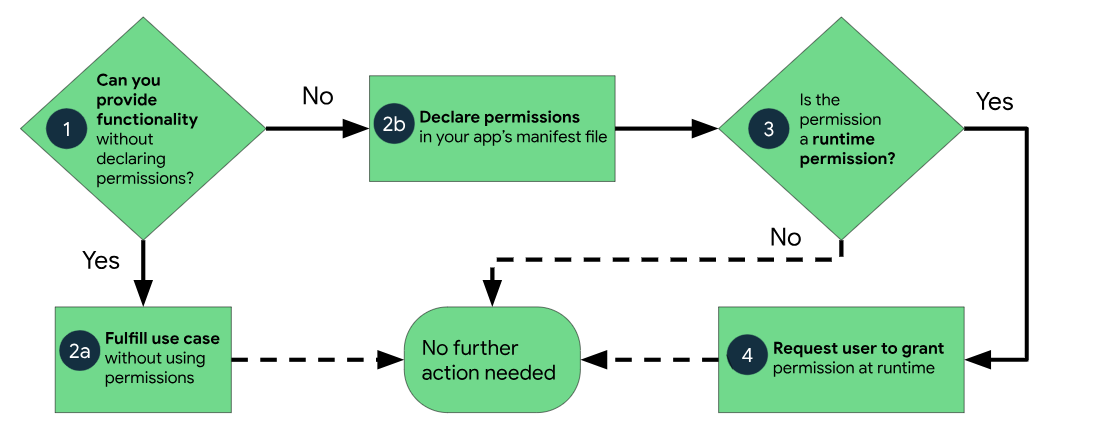
\includegraphics[width=1\textwidth]{images/permission.png}
            \caption{Quy trình sử dụng các quyền trên Android~\cite{runtime-permissions}.}
            \label{fig:android1}
\end{figure} 

